\chapter{Описание АСУ ТП для СК}\label{ch:chn}

\section{Общие слова. Введение в тему}

Автоматизированная система управления технологическим процессом (АСУ ТП) --- это термин,
имеющий отношение к ЭВМ, обеспечивающим управление различными техническими процессами \cite{journal:iter_research_guriev_2016}.
Изначально системы АСУ~ТП использовались исключительно на производстве, но с развитием технологий
и из-за сходства технических процессов АСУ~ТП вышло за рамки управления сугубо производственными процессами
и перешла в другие сферы деятельности, от управления транспортом %\cite{}
до управления техническими процессами зданий %\cite{}
и более сложными техническими сооружениями \cite{journal:vechisl_tech:2004_okolnischnikov}.
%
Далее будет показано создание \todo{аналитической} модели объекта контроля
при создании имитатора объекта контроля и его применение на всех этапах жизненного цикла
объекта контроля: от постановки задачи и проектирования системы контроля, до пусконаладочных работ
и сдачи в опытную эксплуатацию.


Стоит отметить, что для более качественной/глубокой имитации необходимо выделять несколько подмоделей,
анализируя данные этих подмоделей (экспериментально) установить свойства этих подмоделей:
стационарность, детерминированность и проч.

В модели объекта контроля может быть несколько подмоделей \cite{journal:vechisl_tech:2004_okolnischnikov}:
\begin{itemize}
    \item модель технологического объекта управления (правила перехода);
    \item модель имитации внешних сигналов;
    \item модель внутреннего состояния объекта контроля (токи, напряжения и т.д. и т.п.);
    \item \ldots
\end{itemize}

Для пояснения смотри рисунок \ref{fig:submodels_asu_tp}.

\begin{center}
    \begin{figure}[hb]
        % \includegraphics[width=.8\textwidth]{submodels_asu_tp}
        \caption{Структура модели}\label{fig:submodels_asu_tp}
    \end{figure}
\end{center}

Поскольку построение чисто аналитической модели имеет недостаток  в виде отсутствия возможности
описать поведение исследуемого объекта во времени, используется имитационная модель.

\textit{Имитационное моделирование} --- процесс построения некоего алгоритма, который имитирует
поведение исследуемого объекта и взаимодействие исходного объекта с учетом возможных случайных входных величин и
воздействий из внешней среды \cite{book:vvedeni_imit_model_1987}.

Объекты контроля, такие как
    необитаемые автономные подводные аппараты \todo{\ldots},
на которые в любой момент времени возлагается функция готовности к  работе,
нуждаются в проведении проверок при эксплуатации и хранении.
	%
Для проверки ОК необходима система контроля. Создание и отладка СК сопряжена со следующими факторами.
	%
\begin{itemize}
    \item Дороговизна и труднодоступность достаточного количества статистического материала
    натурных испытаний для отладки алгоритмов ПО СК экономически нецелесообразна, так же связана с риском для жизни испытующих.
    %
    \item ОК находится на этапе проектирования.
    %
    \item Отсутствует возможность подключения к ОК.
    %
    \item Проверка граничных значений алгоритмов ОК, ведущих к разрушению ОК недопустима.
\end{itemize}

\chapter{Описание архитектуры имитатора}\label{ch:ch2}

\begin{center}
    \begin{figure}[hb]
        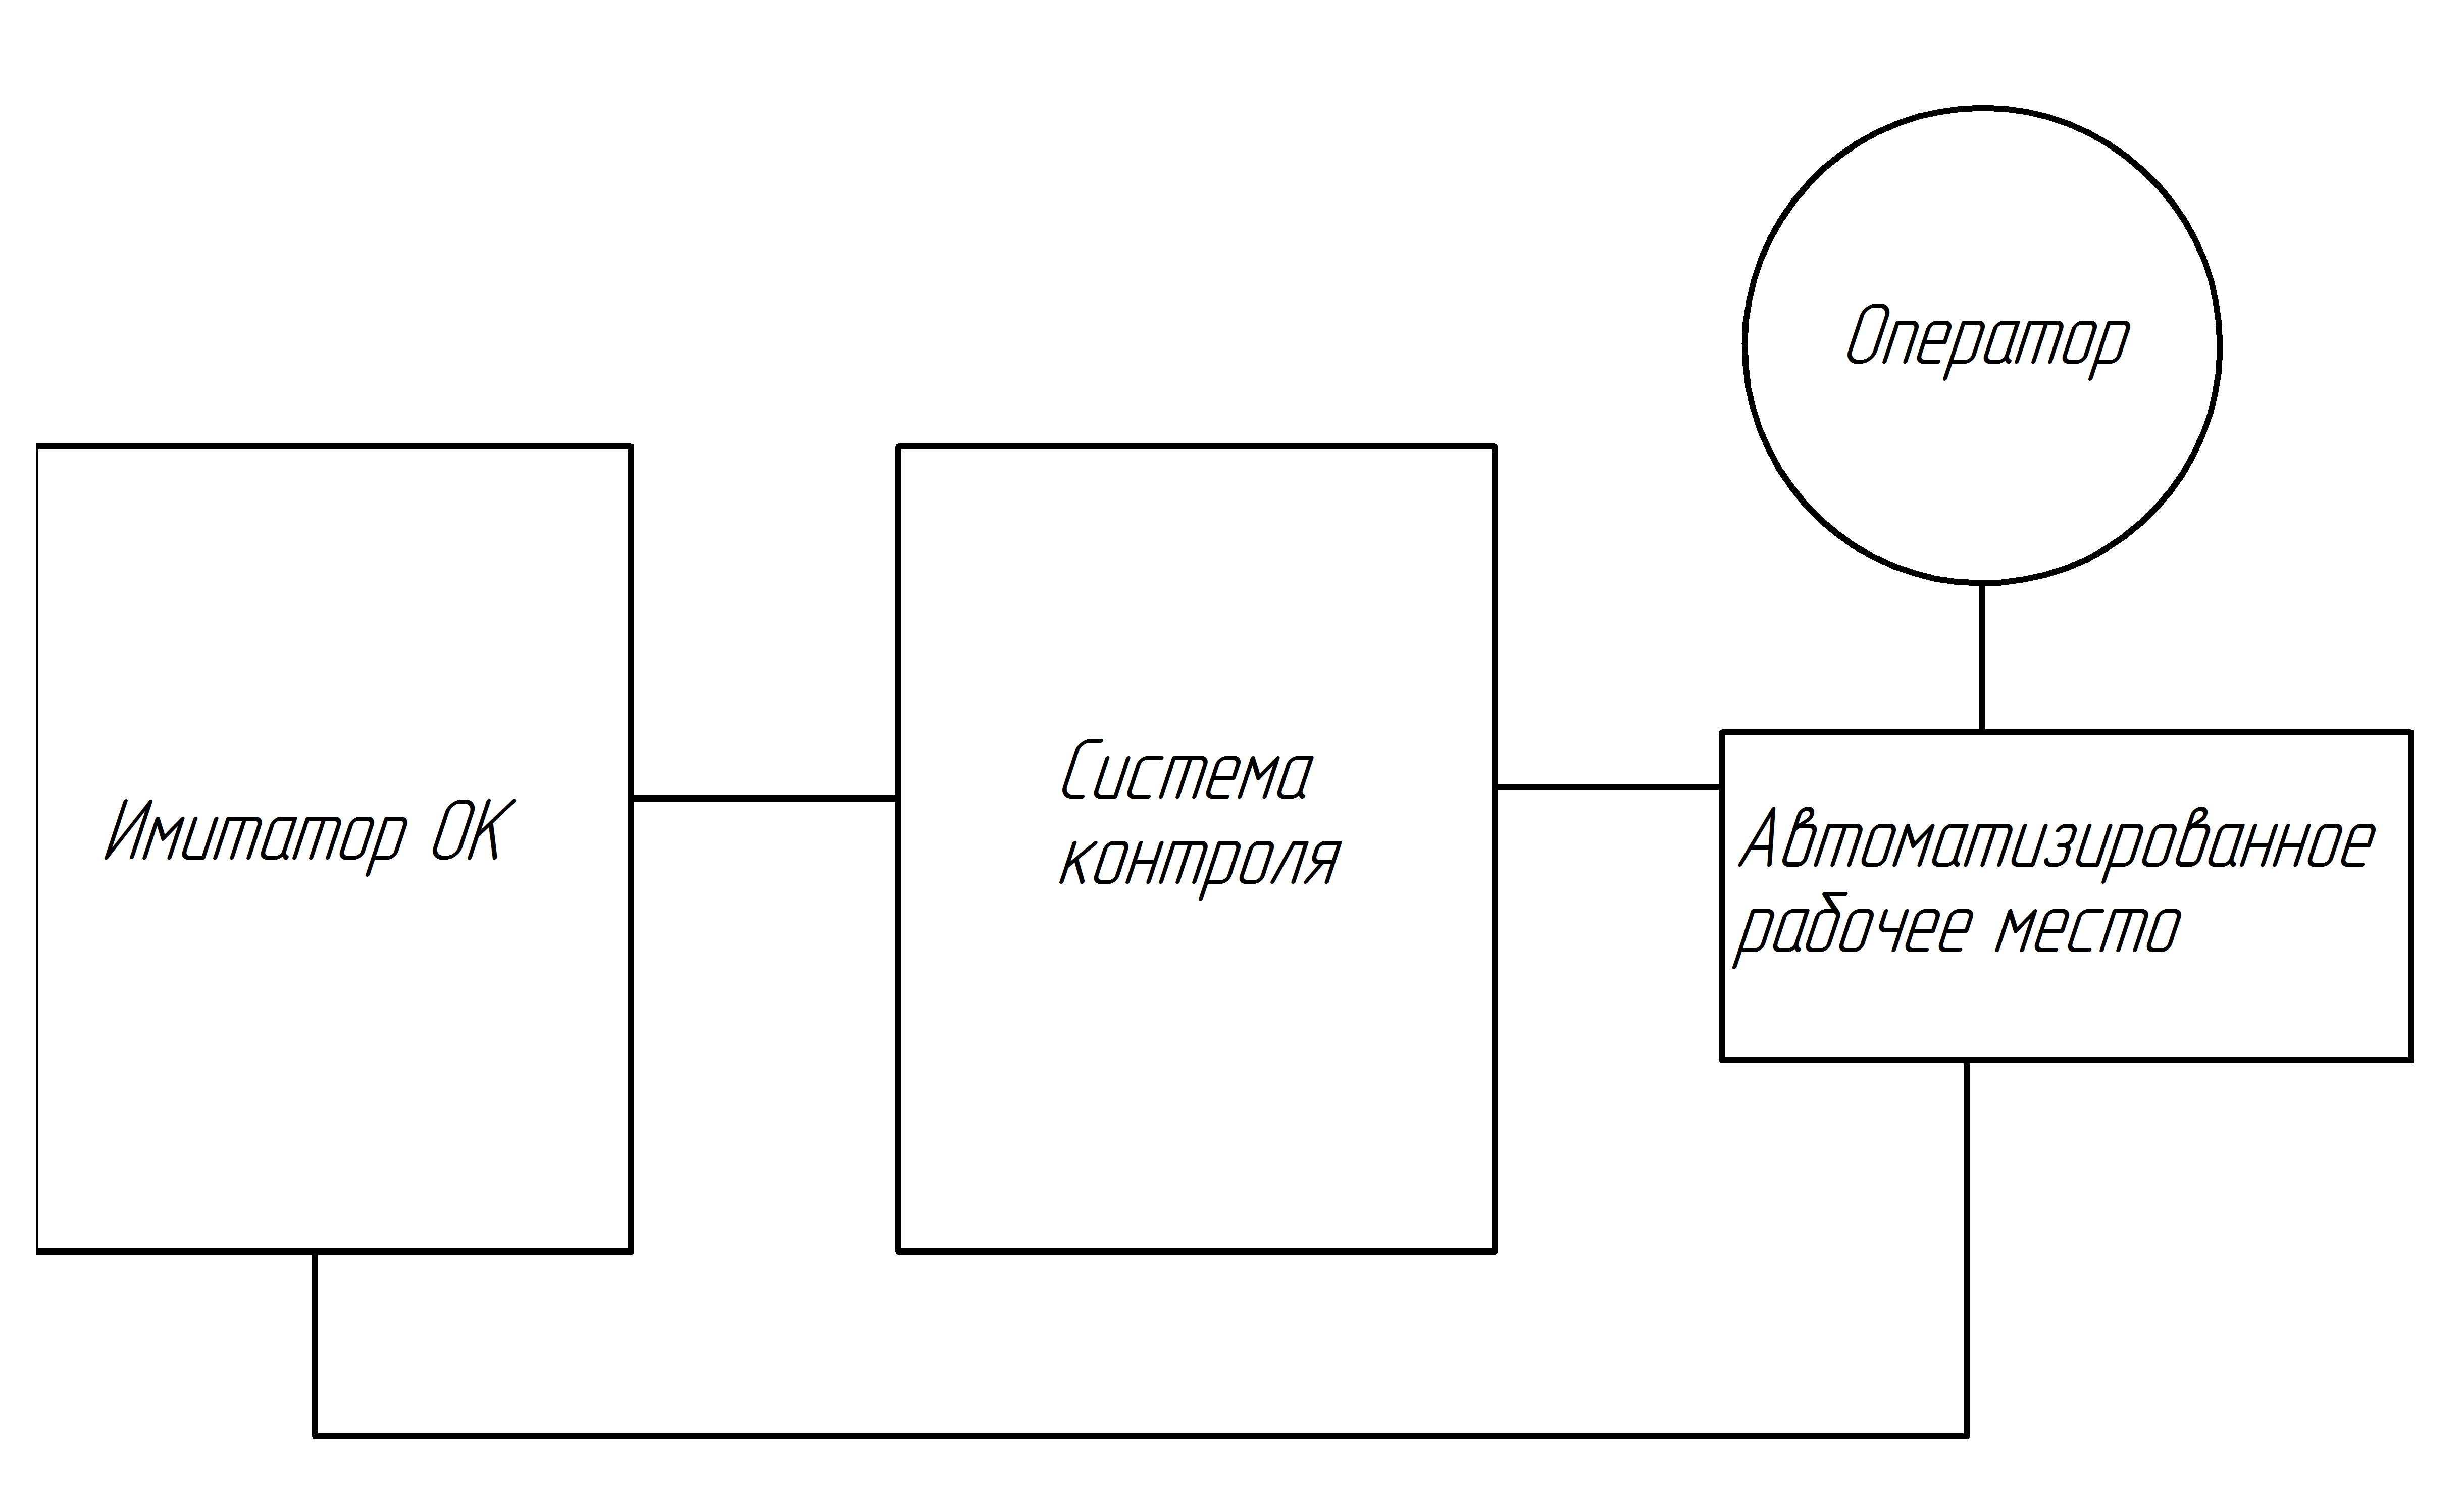
\includegraphics[width=.8\textwidth]{scheme.png}
        \caption{Структура программно-технологического комплекса}\label{fig:asc_schema}
    \end{figure}
\end{center}
    


% \section{Распределение ролей}
% На стороне СК создается экземпляр клиента сети modbus,
% имитатор представляет сервер (см. главу \ref{ch:ch2}).
% \section{Конфигурационный файл}\label{sec:ch2/sec1}
% Общее пространство данных modbus у ПО СК и имитатора \ldots
% \section{Паттерн MVC}
% Поверх множества данных modbus используется паттерн проектирования модель-вид-контроллер \cite{book:pattern:band_of_4}.
% Библиотека Qt позволяет создавать модель данных, наследуя поведение от \lstinline[language=C]!QAbstractTableModel!,
% переобпределяя реализацию методов для чтения-записи данных в модель.
% \subsection{Пояснение в реализации методов}
% \subsection{Преимущества такого подхода}
